%
% File acl2012.tex
%
% Contact: Maggie Li (cswjli@comp.polyu.edu.hk), Michael White (mwhite@ling.osu.edu)
%%
%% Based on the style files for ACL2008 by Joakim Nivre and Noah Smith
%% and that of ACL2010 by Jing-Shin Chang and Philipp Koehn


\documentclass[11pt]{article}
\usepackage{acl2012}
\usepackage{times}
\usepackage{latexsym}
\usepackage{amsmath}
\usepackage{graphicx}
\usepackage{multirow}
\usepackage{enumerate}
\usepackage{url}
\DeclareMathOperator*{\argmax}{arg\,max}
\setlength\titlebox{3.5cm}    % Expanding the titlebox
\newcommand{\ignore}[1]{}

%\newcommand{\B}{\mathcal{B}} 

\title{A Model of Random Walks on Bipartite Graph for Classification Problems}

\ignore{
\author{First Author \\
}
}

\date{}

\begin{document}
\maketitle
\begin{abstract}
We introduce a general framework of semi-supervised graphical model that is
applicable to any classification tasks that can be represented with norminal
features, requiring only a handhul of labeled examples.
We conducted experiments on three different NLP tasks: prepositional phrase 
attachment, named entity classification, and domain-specific terminology extraction. 
We show both theoretically and empirically how the graph structure helps making 
use of large amount of unlabeled data.
Based on the empirically study of underlying correlations between graph structures and
classification performance, we incorporate active learning techniques to 
achieve the best learning rate with minimum requirement on labeled data. 
\end{abstract}

%%%%%%%%%%%%%%%%%%%%%
\section{Introduction}

Semi-supervised learning on graphs is a direction that has drawn great
attentions from NLP researchers. %The general idea behind various semi-supervised
%graphical methods is constructing a graph can be automated, while 
An abstract framework that we have often seen in graph based NLP is constructing
a graph in which each vertex represents an instance which can
be a word, a concept, a sentence, an article etc. Edges
are connected and weighted according to some manually selected
function that defines the closeness or similarity of any two instances in the
context of the application. 
One possible usage of the graph is to predict the
property (label) of a node via comparing the distances of this node to other
nodes with known labels. For example, //add a citation here

Another information we can obtain from the graph is the importance of a node.
We see algorithms such as PageRank\cite{}, HITS\cite{}, and graph based
summarization systems\cite{} .




In this paper, we introduce a model that shares with many other graphical
methods the idea of encoding similarities between instances into a graphical
structure and learning from unlabeled instances, while presents its novelty in
the following two aspects. First, the graph is bipartite. Example nodes and
feature nodes form two subsets of the bipartite graph. We will show later this
can be equivalently converted to a graph consisting of only example nodes
assuming a special edge weight definition. This
assumption simplifies the graph construction by a factor of the number of example nodes. 
Second, we observe from experiment that when the labeled training size is very
small compared to the entire graph, performance of the model is unstable due to the
randomness in sampling training examples. We extend the model with an active
learning technique that intellegently chooses the most ``informative'' unlabeled
examples to learn. Such property is well appreciated in applications where
labeled examples are very expensive to obtain.  


%%%%%%%%%%%%%%%%%%%%%
\section{An Overview of Semi-Supervised Learning on Graphs}

%It is also known as transductive learning, when the instances of
%interest are limited to the unlabeled instances observable at training stage, in
%other words, the predictor does not need to deal with future test data.
Semi-supervised learning uses both labeled instances and unlabeled instances as
training data. 
Typically the unlabeled data size is much larger than labeled data size. The
learning aims at predicting the labels for unlabeled data.

\subsection{Graph Construction} \label{sec:graphconst}
Graph-based SSL represents the labeled and unlabeled instances\footnote{We use
the term ``instance'' and ``example'' interchangabally in this paper.} jointly on a
graph as nodes. Suppose there is a set of 
$n$ examples, among which $l$ are labeled, $u$ are unlabeled;
$n = l + u$, usually $n >> l$.\footnote{Notations introduced in this section will be used throughout
the paper.}
Denote $L$ the labeled example set and $U$ the unlabeled example set.

$L:= \{(x_1, y_1), (x_2, y_2), ..., (x_l, y_l)\}$;

$U:= \{x_{l+1}, x_{l+2}, ... x_{l+u}\}$.

Edges are usually undirected, representing the similarity of two instances.
Denote the edge weight connecting two nodes $x_i$ and $x_j$ as
$w_{ij}$, there can be several types of graph encoding the edge weights:

\textbf{Fully connected graph.} Eedge weight is defined by the Gaussian
kernel, also known as Radial Basis Function (RBF) kernel: \[ w_{ij} =
exp(- (\|x_i-x_j\|^2/2\sigma ^2) \]
The edge weight decreases as the Euclidean distance of the two nodes
increases, with rate depending on the parameter $\sigma$.

\textbf{$\epsilon$NN graph.} 
$\epsilon$ is the threshold distance value for two nodes to be connected
by an edge. In the unweighted setting, \( w_{ij} = 1 \mbox{ if } \|x_i-x_j\| \leq
\epsilon \mbox{ and } 0 \mbox{ otherwise }\).

%        Use of $\epsilon$NN graph needs the graph to be uniformly scaled over
%        the data space. If the graph contains data points of different scales in
%        different regions, $\epsilon$NN graph faces the difficulty of choosing
%        effective parameter  $\epsilon$. 

\textbf{kNN graph.} Every node links to the $k$ nearest neighbors in Euclidean
distance. The edges can either be unweighted 
       % (i.e. edge weight is $1$ if
       % two nodes are connected and $0$ otherwise),
or weighted using the Gaussian kernel function defined above. 
       % However, the neighborhood
       % relationship is not symmetric. There can be two nodes $i, j$ that $j$ is
       % among the k nearest neighbors of $i$ while $i$ is not among the k
       % nearest neighbors of $j$.
The common definition of a kNN graph connects
$i, j$ if the kNN relationship exists in at least one direction.
%        Thus
%        the average degree of a kNN graph is usually larger than k. As opposed
%        to  $\epsilon$NN graph, kNN graph can connect points on different
%        scales. It is possible to have connected nodes in two relatively far
%        away clusters of different densities.

%         An alternative construction is called \emph{mutual kNN graph}, where
%         edges exist only when two nodes have kNN relationship mutually. Mutual
%         kNN graph has the property in between kNN graph and $\epsilon$NN graph.
%         It connects nodes within regions of constant density but does not
%         connect regions of different density scales together and is thus suited
%         for detecting clusters of different densities.





Apart from the choice of weighting, a more substantial pre-requisite for all
graph-based learning methods is a well chosen feature space and an effective
similarity function, so that the "neighborhoods" deduced from the similarity
or distance metric are meaningful.  
This is however, often difficult to practice in NLP tasks because of the
discrete or heterogeneous feature spaces.
How to select features and possibly project the features
into a subspace is still an under-investigated problem \cite{alex}.


\subsection{Mincut}\label{sec:mincut}

Blum and Chawla first formulated an SSL algorithm as a graph cut problem in
\cite{blum}. In the binary classification case, each positive labeled instance
acts as ``source'' and negative labeled instance acts as ``sink''.
A cut is defined as a set of edges whose removal
blocks the flow from ``sources'' to ``sinks''.
The Mincut algorithm aims at finding the cut whose
edge weight sum is the minimum.
Utilizing the Ford-Fulkerson method for computing Max Flow, it is solvable in polynomial time. 
The learned predictor assigns
positive label to every unlabeled node that ends up in the same component with
positive labeled examples, and vice versa. 

Mincut is based on a Marcov random field
assumption. Edge weights represent the Markov transition probability between
nodes, thus similar nodes have higher edge weights. The binary label case is
equivalent to Boltzmann machine. Formalizing Mincut as a regularized risk
minimization problem, we minimize the sum of a loss function and a regularizer.
Suppose binary labels $1$ and $0$, the loss function is \[ \infty  \sum_{i\in
L} (y_i - f(x_i))^2\]
The infinity weight forces the labeled data to be fixed at their given labels.
The regularizer is 
\begin{equation}\label{eq:mincut}
    \frac{1}{2}\sum_{i,j=1}^{u+l}w_{ij}(f(x_i)-f(x_j))^2 \mbox{, where
    }f(x_i)\in\{0,1\}\end{equation}
    corresponding to the cut size. 


\subsubsection*{Variants of Mincut}
    There are two drawbacks for the plain Mincut method.
    First, the infinity weight in loss function forces a ``hard cut'' -- labeled
    data are fixed at the original labels, unable to handle noises in labeled
    data.  
    Second, there's no guarantee for balanced cut in sense of resulting class
    size. When multiple minimum cuts exist, the algorithm always returns the
    first solution,
    %Due to the working mechanism of its algorithm, this
    %solution is the nearest to one class of labels,
    which is often not the
    optimal one from the practice perspective. 

    To address these problems, \cite{blum2} extend the plain
    Mincut by randomizing the graph structure. They
    disturb the graph by adding artificial random noise to edge weights, then
    solve the Mincut on resulting graphs. 

    RatioCut \cite{ratiocut} and NCut \cite{shi}
    circumvent the problem of unbalanced cut. Ratiocut measure class balance in
    terms of class size, while NCut balances edge weights.
    \begin{equation}\label{eq:ratiocut}
        RatioCut(A, B) =  \frac{ \sum_{i \in A, j \in B} w_{ij}}{ |A|} +
        \frac{ \sum_{i \in B, j \in A} w_{ij}}{ |B|}
    \end{equation}

    \begin{equation}\label{eq:ncut}
        NCut(A, B) =  \frac{ \sum_{i \in A, j \in B} w_{ij}}{ \sum_{i \in
        A} d_i} + \frac{ \sum_{i \in B, j \in A} w_{ij}}{\sum_{i \in B} d_i},
    \end{equation}
    where the degree of node $x_i$ is defined as  $d_i =
    \sum_{j=i}^{n}w_{ij}$.



    \subsection{Harmonic Function and Gaussian Fields}

%1) Relation to Zhu's method harmonic function and Gaussian fields
%
%-- distribution assumption
%
%Zhu's method assumes Gaussian random fields, the propability distribution of random
%walk is a continuous Gaussian distribution on the reverse of the distance
%between any two nodes. The graph is fully connected. 
%
%
%It is a good model when the geometric distance is well defined.
%
%In the bipartite graph model, the propability of one random step is propotional to the number of
%common features shared by the two example nodes. It is actually the dot product
%of two examples (recall that an example is a vector of dimention $m$).
%If the number of features connected to every example 
%is same, i.e. every example has same magnitude, like in the pp attachment case,
%then it's also cosine). The random walk propability is a discrete distribution.
%
%-- advantage of tumbl
%
%graph construction is cheap: $O(nm)$, Zhu's method needs
%to compute a $n \times n$ weight matrix, where each entry contains calculation
%of distance, so the complexity is $O(n^2m)$
%
%
    \cite{zhu03} applies Gaussian random fields on a graph consisting of
    labeled and unlabeled instances. Edges are weighted using the RBF kernel.
    The method shares the same assumption with other graph-based methods like 
    nearest neighbor and mincuts, that similar examples should belong
    to same class. The difference is the Gaussian field is a continuous space,
    rather than discreet space over the unlabeled nodes. 

    If we express the regularization using the loss function and regularizer,
    we find it has the same loss function as Mincut,  \[ \infty
    \sum_{i\in L} (y_i - f(x_i))^2 \]  which fixes labeled data at given labels. The
    regularizer (equation \ref{eq:reg}) is based on the graph combinatorial Laplacian $L$ 
    \ref{sec:spec}), with an important relaxation that $f_i \in (0, 1)$, instead
    of $f_i \in \{0,1\}$ as in Mincut.

    \begin{equation} \label{eq:reg}
        \frac{1}{2} \sum_{i,j=1}^{u+l}w_{ij}(f(x_i)-f(x_j))^2 =   f^T L f 
    \end{equation}

    The solution to the problem is a harmonic function that has a closed form
    solution easily computed by matrix calculation. It also has the ``harmonic''
    property as in equation \ref{eq:har}.
    \begin{equation} \label{eq:har}
    f(j) = \frac{1}{\sum_i w_{ij}}}\sum_{i\in Neighbor(j)} w_{ij} f(i),\end{equation}
    \[
        \mbox{for }j=l+1, l+2, ..., l+u
    \]      
    This provides the theoretical support that iterative label propagation algorithm
    converges to the harmonic function solution.

    \subsubsection*{Connection to random walks}

    On the same graph, a random walker starts from node $x_i$. We can define the
    probability of stepping to node $x_j$  in the next move be the normalized
    weight $w_{ij}$. If we assign 0 and 1 to the two classes
    of labeled examples, the harmonic function's solution at node $x_i$: $f(x_i)$
    is the probability for a random walker starting from $x_i$ and hitting an
    example labeled $1$ before hitting a $0$.

%
%    We can also build an electrical circuit to simulate the harmonic energy
%    minimization procedure. Nodes in the graph are transformed to nodes of
%    the electrical network, edge weights represent the conductance (the
%    inverse of resistance) between each pair of nodes. If we apply 1 Volt
%    voltage to all the labeled nodes of one class, and connect the other
%    class of labeled nodes to ground, the circuit will finally stable at an
%    equilibrium state, which minimizes energy dissipation. The electric
%    potentials for each node in the steady state are exactly the solution to
%    the harmonic function.
%









    \subsection{Spectral Methods}\label{sec:spec}
Spectral clustering is an unsupervised graph method. The central role of graph
Laplacian connects several methods in previous section from the spectral theory
view. We first look at the formal definitions of normalized, unnormalized graph
Laplacian and their properties. The rest of the section discusses some points of
view that connect spectral clustering with other graph methods.

\subsubsection*{Graph Laplacian}\label{sec:specdef}


We will be using the following notations to describe an undirected graph $G = (V, E)$:\\
The node set $V = {x_1, ..., x_n}$;\\
The adjacency matrix $W = (w_{ij} ) _{i,j = 1, ..., n} $;\\
The degree of $x_i$, $d_i = \sum_{j=i}^{n}w_{ij}$;\\
The degree matrix D is the diagonal matrix with degrees $d_1, ..., d_n$ on the diagonal;\\

The unnormalized graph Laplacian is defined as \[L=D-W\] For every function $f: [n]\rightarrow \mathbb{R}  $,
\begin{equation} 
f^T L f = \frac{1}{2} \sum_{i,j=1}^{n}w_{ij}(f(x_i)-f(x_j))^2
\end{equation}
It's trivially proved that $L$ is positive semi-definite and symmetric. 
It follows that $L$ has n non-negative eigenvalues, $0 = \lambda_1\leq \lambda_2 \leq ... \leq \lambda_n$. We denote their corresponding eigenvectors $\phi_1, ..., \phi_n$. The spectral decomposition is $L = \sum_{i=1}^n \lambda_i\phi_i\phi_i^T$.

An important property used in spectral clustering is that the number of zero eigenvalues equals the number of connected components in the graph.\\

The normalized graph Laplacian is defined as \[ \mathcal{L} = \mathbf{I} - D^{-1\/2}W D^{-1\/2}\]
For every function  $f: [n]\rightarrow \mathbb{R}  $,

\begin{equation} 
f^T \mathcal{L} f = \frac{1}{2} \sum_{i,j=1}^{n}w_{ij}(\frac{f(x_i)}{\sqrt{d_i}}-\frac{f(x_j)}{\sqrt{d_j}})^2
\end{equation}
The properties of $L$ discussed above apply to $ \mathcal{L}$.
\par
Graph Laplacian in SSL is used to encode the smoothness of function $f$.   For
example, $f^T L f$ can be used as a regularizer in transductive classification
since a low value of  $f^T L f$ requires $f$ changing very little in high
density regions.  In other words, $f^T L f$ makes a ``cluster assumption'' that
decision boundary of a classifier lies in low density regions.

\subsubsection*{Spectral clustering algorithm}\label{sec:specalg}
The spectral clustering works as follows: From the first $k$ eigenvectors of $L$,
$\phi_1, ..., \phi_k$, we span a new space $V \in \mathbb{R}^{n\times k}$ which
contains the $k$ eigenvectors as columns. Then the data points are mapped to the
rows of $V$, i.e., for $i = 1, ..., n$, the projection of data point $x_i$ is
the $i$-th row of $V$. We then perform clustering using traditional methods such as
k-means on the new projections of data points.
%
%Shi and Malik\cite{shi} propose a normalized spectral clustering algorithm, where instead of using the first k eigenvectors of $L$,  they use the k eigenvectors of the generalized eigen problem $L\phi = \lambda D \phi$.  Another way of normalization (Ng et al.\cite{ng2}) uses normalized graph Laplacian $\mathcal{L}$ to compute the k eigenvetors, and normalize the matrix $V$ to such that the row sums have norm $\mathbf{1}$.
%
%\subsubsection{Spectral clustering in practice}
%As has been stated before, the effectiveness of similarity function encoded in  $W$ is substantial to the performance of all graph-based methods, which is beyond the discussion of this section. In additional, spectral clustering is also very sensitive to the choice of graph type and parameters \cite{luxburg} (section \ref{sec:graphconst}).
%
%A general problem for unsupervised clustering is how to determine the number of clusters $k$.  The common approach is the eigengap heuristic. In the ideal case when we have $k$  disconnected subgraphs, the clustering is easily solved by  finding the $k$ zero eigenvectors. When the clusters are not perfectly separated (links exist between clusters), we find the eigenvector $\phi_k$ such that $\phi_{k+1} - \phi_{k}$ is relatively large. The eigengap heuristic indicates the data set contains $k$ clusters.
\subsubsection*{Connection with Graph Cut}

Recall that Mincut can be interpreted as a problem of minimizing the objective function (\ref{eq:mincut}) with the constraints of $f$ being discrete labels and consistent with clamped labels. 

Consider the RatioCut objective function (\ref{eq:ratiocut}), we define $f$    
\begin{equation}\label{eq:fi}  
f(x_i) = \left\{ \begin{array}{ll}
\sqrt{|B|/|A|} & \mbox{if }x_i \in A \\
\sqrt{|A|/|B|} & \mbox{if }x_i \in B \end{array} \right. \end{equation}
and thus can rewrite 

\begin{align} 
    f^TLf & = \frac{1}{2}\sum_{i,j=1}^{n}w_{ij}(f(x_i)-f(x_j))^2 \\
    &= |V|\cdot RatioCut(A, B)
\end{align}

If we relax the constraints $f$ being a binary function to real numbers, we are
able to use the above equation to approximate the problem of minimizing  $
RatioCut(A, B)$ to minimizing $ f^TLf$ subject to constraint (\ref{eq:fi}),
which is equivalent to $f \bot \mathbb{1}$ and $\|f\| = \sqrt{n}$. The solution
of the relaxed problem is the second eigenvector of $L$. The real-valued
solutions can easily be transformed to labels or classes by taking threshold $0$.

Following similar lines of calculations we can show that relaxed Normalized Ncut
defined by (\ref{eq:ncut}) can be approximated by normalized spectral
clustering \cite{shi}.

\subsubsection*{Connection with Random Walk}

From the random walk point of view, we define the transition matrix $P$ as
\[P = D^{-1}W\]
The stationary probability $\pi_i = d_i/\sum_{j,k=1}^{n} w_{jk}$ is unique if
the graph is connected and non-bipartite. For disjoint subset $A$,$ B$, denote
$P(B|A)$ as the the probability of a random walk starting with a node in $A$
ends at a node in $B$. It has been proved that \[Ncut(A, B) = P(A|B) + P(B|A)\].
We thus can interprete the problem of minimizing Ncut equivalently as a
partition of the graph such that random walks seldom transit across different
classes. This consequently relates random walks to the normalized graph
Laplacian.

Another concept that connects random walks with graph Laplacian is the commute
distance. The commute distance is the expected time it takes for a random walker
starting at $x_i$ to travel to $x_j$ and then back to $x_i$.  
Nodes are closer if there exist multiple
paths so the commute distances are shorter in dense regions. The commute
distance can be computed from the generalized inverse of the graph Laplacian
$L$ \cite{klein}. 

%\subsubsection{Spectual Method in SSL: Spectual Graph Transducer}
%
%Joachims\cite{sgt} introduces the transductive version of k-NN graph and the Spectral Graph Transducer (SGT), which uses spectral Laplacian to effectively solve the k-NN problem. It also provides a general review of several SSL approaches: transductive SVM, s-t mincuts and Co-trainig. Their connections, strengths and drawbacks are discussed.
%Experiment results of TSVM, kNN, SGT on six datasets are reported.
%\par
%Pham et al.~\cite{pham} later applied the SGT algorithm to WSD and combined it with co-training.
%


%%%%%%%%%%%%%%%%%%%%%

\begin{figure*}[ht!]
\centering
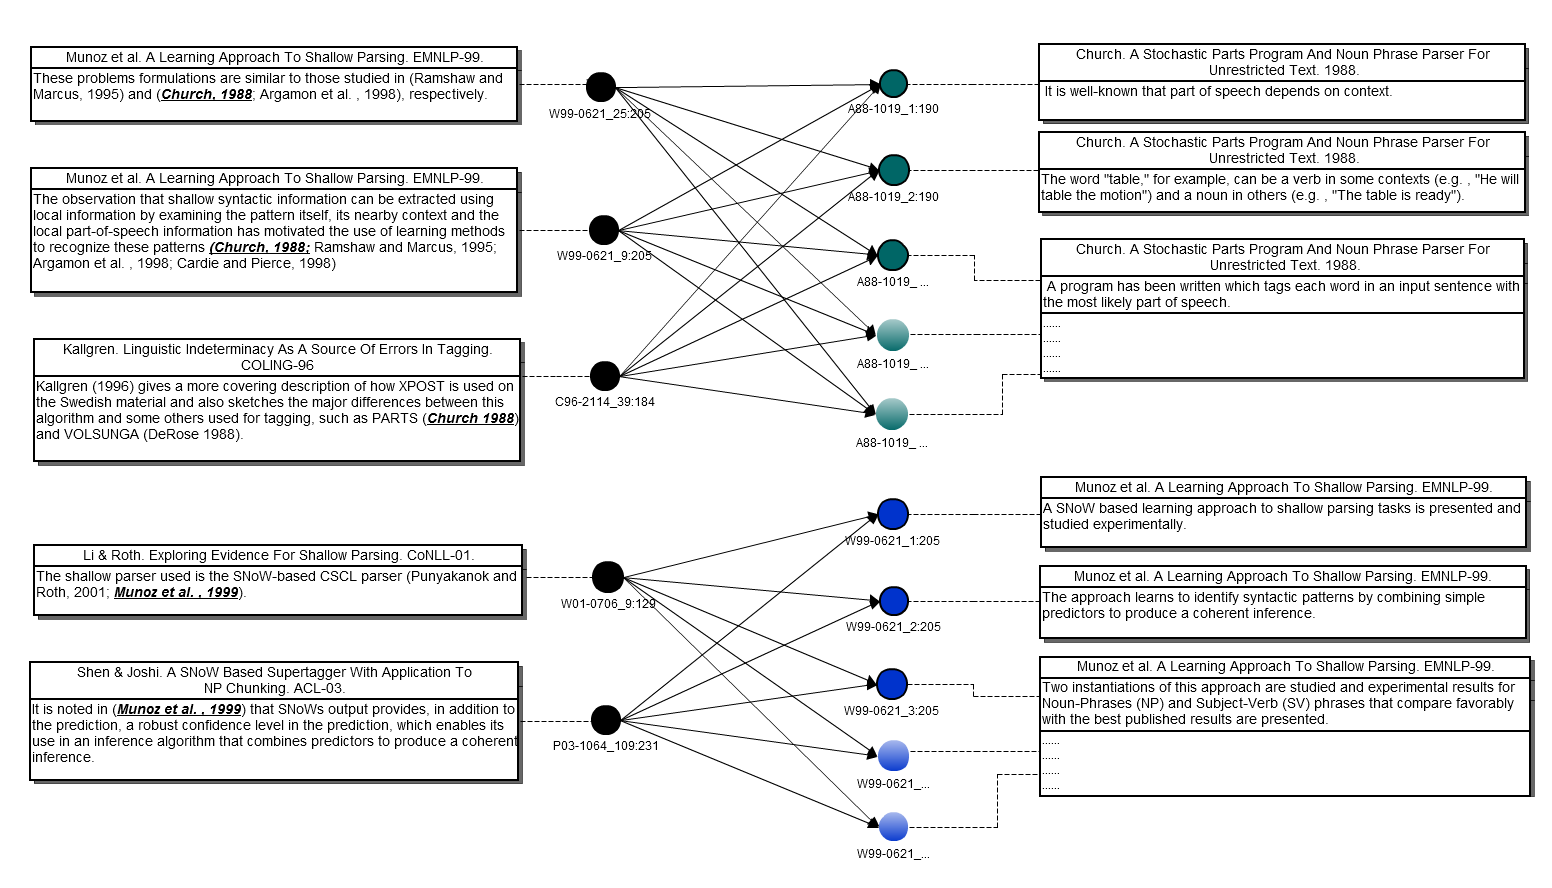
\includegraphics[width=\textwidth]{graph/bipartite_graph.png}
\caption{A mini-model of the bi-partite graph for Chapter 5 (Part-of-Speech Tagging)}\label{fig:bi}
\end{figure*}

\begin{table*}
\centering
{\scriptsize
\begin{tabular}{|l|cc|rrr|}
  \hline
 Chapter & src & cit & $|\B_L|$ & $|\B_R|$ & $E_\B$ \\
  \hline \hline
 Words and Transducers & 14&     255&    489&    $3,484$ &   $202,940$ \\
 N-grams & 5&      73&     97&     $2,083$ &   $32,690$ \\
 Part-of-Speech Tagging & 16&     657&    $1,261$ &   $3,385$ &   $344,886$\\
 Hidden Markov and Maximum Entropy Models & 2&      432&    659&    525&    $187,905$\\
 Phonetics & 1&      12&     81&     216&    $17,496$\\
 Speech Synthesis & 4&      54&     126&    920&    $29,357$\\
 Automatic Speech Recognition & 2&      27&     103&    401&    $21,566$\\
 Speech Recognition: Advanced Topics & 7&      189&    445&    $2,007$&   $96,467$\\
 Syntactic Parsing & 4&      131&    246&    763&    $63,673$\\
 Dialog and Conversational Agents & 11&     170&    368&    $3,745$ &   $114,281$\\
  \hline
\end{tabular}}
\caption{List of chapter historical notes used in our experiments together with the number of source papers extracted from historical notes (src), the number of citing papers extracted from AAN (cit), size of the left ($\B_L$) and right ($\B_R$) components in the bi-partite graph, and number of edges in the graph ($E_\B$).}\label{tbl:chapters}
\end{table*}

\section{Approach}
\label{sec:approach}

Previous work on scientific survey generation have compared surveys that are generated from different sources such as citations and source paper texts~\cite{Qazvinian&Radev08a,mei&zhai08,mohammad-EtAl:2009:NAACLHLT09}. However, none of these approaches combine these heterogeneous information sources to produce automatic surveys. 

In our approach, we investigate the usefulness of combining different information sources and producing summaries that are both affected by source paper text and citation information. For a set of papers in the same scientific topic, we extract survey worthy sentences from the source texts that cover contributions recognized by other scholars in citations, and extract citations that cover contributions that are recognized by the authors in the source text.

In our algorithm, we model the set of papers in a scientific topic $t$ as a bi-partite graph, $\B$ with a left and a right component ($\B_L$, $\B_R$). Each node in $\B_L$ is a citation sentence to one or more papers in $t$ extracted from AAN, and each node in $\B_R$, represents a sentence extracted from the source text of a paper in $t$. We construct the edges in $\B$ by connecting each citing sentence to all the source sentences in the papers it cites. Each edge in $\B$ is assigned a weight equal to the cosine similarity of the TF-IDF term vectors of the two sentences it connects. 
Figure~\ref{fig:bi} illustrates part of the bi-partite graph for built for the ``Part-of-Speech Tagging'' chapter in the JM book.

To build the summaries we are interested in citations and source sentences that cover important contributions in the given scientific topics. Intuitively, contributions that both the paper authors and other scholars recognize as significant are important and should be extracted. Surveyor extracts citations that cover important contributions mentioned in the source papers as well as source sentences that discuss important factoids recognized by others in citations.


\subsection{Ranking}
The inherent duality in the source papers and citations suggests that the problem could be addressed by applying the HITS algorithm~\cite{Kleinberg:1999} to iteratively assign hub and authority scores to citations and source sentences respectively. The induction process is as follows. Each citation sentence $c\in \B_L$ is associated with a hub score $h_c$, and each source sentence $s\in \B_R$ is associated with an authority score $a_s$. These scores are initialized with a value of $1.0$.  Hub and authority scores are iteratively updated using the following equations.

{\small
\begin{eqnarray}
\label{hits1} a^{(i+1)}_s = \sum_{c\in nei(s)} \frac{h^{(i)}_c}{H^{(i)}}
\end{eqnarray}
}
{\small
\begin{eqnarray}
\label{hits2} h^{(i+1)}_c = \sum_{s\in nei(c)} \frac{a^{(i)}_s}{A^{(i)}}
\end{eqnarray}
}

where a source sentence $s$ is in a citation sentence, $c$'s neighborhood ($s\in nei(c)$) if there is an edge between $s$ and $c$ in $\B$ ($c$ cites the paper that contains $s$), and their cosine similarity is greater than a threshold (i.e., $cos(s,c) > \theta$). Here, $H^{(i)}$ and $A^{(i)}$ are normalization factors:

{\small
\begin{eqnarray}
H^{(i)} = (\sum_{c\in \B_L} {h^{(i)}_c}^2)^{1/2}\\
A^{(i)} = (\sum_{s\in \B_R} {a^{(i)}_s}^2)^{1/2}
\end{eqnarray}}

In our experiments, we set $\theta = 0.1$. This ranking gives us top authorities (source sentences) and top hubs (citations) with which we build two different summaries: {\bf $\textrm{HITS}_\textrm{src}$} and {\bf $\textrm{HITS}_\textrm{cit}$}. Although these summaries are built from different sources (i.e., source papers and citations) they are affected by each other. In other words, the scores and thus extraction of top citations affects the extraction of top source sentences and vice versa. 


\subsection{Adding Weights}
In previous section, we described the basic version of our system in which the edges are considered as binary connections (if the cosine similarity is above a threshold). We would like to investigate the effect of similarity on sentence extraction. In other words, instead of applying a threshold we use the actual edge weights and modify Equations \ref{hits1}, \ref{hits2} as follows.

{\small
\begin{eqnarray}
\label{whits1} a^{(i+1)}_s = \sum_{c\in nei(s)} \frac{w_{cs} \cdot  h^{(i)}_c}{H^{(i)}}\\
\label{whits2} h^{(i+1)}_c = \sum_{s\in nei(c)} \frac{w_{sc} \cdot a^{(i)}_s}{A^{(i)}}
\end{eqnarray}}

where $w_{sc}$ is the is the edge weight between vertices $s$ and $c$, calculated as the TF-IDF based cosine similarity between their corresponding sentences.

Intuitively, this modification will take into account the similarity of sentence with its neighbors rather than the number of connections, and would result in summaries that contain more \emph{lexically} salient sentences. 
The weighted ranking gives us top authorities (source sentences) and top hubs (citations) with which we build two different summaries: {\bf $\textrm{HITS}_\textrm{src} \textrm{ with weights}$} and {\bf $\textrm{HITS}_\textrm{cit} \textrm{with weights}$}.

\subsection{Citation Bias}
The downside of the current HITS-based sentence extraction is that it assumes equal importance for the papers in a given topic. However, contributions from highly cited papers are intuitively more important. To address this issue, we propose an improvement inspired by~\cite{Mei&al2010} and modify equations \ref{hits1}, \ref{hits2} to include a prior distribution of prestige.

{\small
\begin{eqnarray}
\label{phits1} a^{(i+1)}_s = (1- \lambda) \cdot p^\ast(s) + \lambda \cdot \sum_{c\in nei(s)} \frac{h^{(i)}_c}{H^{(i)}}\\
\label{phits2} h^{(i+1)}_c = (1- \lambda) \cdot p^\ast(c) + \lambda \cdot \sum_{s\in nei(c)} \frac{a^{(i)}_s}{A^{(i)}}
\end{eqnarray}}

Here, $p^\ast(v)$ is a distribution which represents the prior preference of vertex $v$. When $p^\ast(v)$ is uniform, the left component is similar to the random jumping probabilities in PageRank. Other possible choices for $p^\ast(v)$ include a topic sensitive distribution, inspired by personalized jumping in personalized PageRank~\cite{Haveliwala2002,haveliwala2003topic}. 
In Equations~\ref{phits1},~\ref{phits2} $\lambda$ obtains a value between $0$ and $1$. When $\lambda = 1$, Equations~\ref{phits1},~\ref{phits2} lead to the standard HITS algorithm. In our experiments, we set $\lambda = 0.75$. 

The prior distribution allows us to favor citation sentences that are from more impactful papers. Therefore we define the prior distributions as the normalized citation frequency of the paper 

{\small
\begin{eqnarray}
p^\ast (v) = \frac{C_v + 1}{\sum_{v\in \B} C_v + |\B|} 
\end{eqnarray}}

where $C_v$ is the number of citations to the paper that contains sentence $v$.  
Equations~\ref{phits1},~\ref{phits2} give us top authorities (source sentences) and top hubs (citations) with which we build two different summaries:  {\bf $\textrm{HITS}_\textrm{src} \textrm{ with priors}$} and {\bf $\textrm{HITS}_\textrm{cit} \textrm{with priors}$}. 


%%%%%%%%%%%%%%%%%%%%%
\section{Active Learning}


Observations in a pilot experiment on the
preporsitional phrase attachment dataset motivated applying 
active learning.
In this section, we first briefly describe the PP
attachment classification task, dataset, and results form the pilot experiment.
Then we present the active learning algorithm.

\subsection{PP Attachment Dataset}\label{ppdata}

1) ppattach disambiguation

2) dataset

3) state-of-art, backoff method

\subsection{Pilot Experiment}

use basic tumbl model

plot: learning curve from 10 to 1000 training size 

plot: uncertianty - when sample size is small (e.g. 10 , 50) performance

variance is large, motivate a method to better choose examples to be labeled


\subsection{Algorithm with Active Learning}

// need to fill in after experiments



\section{Experiments} \lable{sec:experiment}

\subsection{PP attachemnt dataset}


1) baseline: backoff method

2) tumbl, randomly pick labeled examples

3) active learning

Todo: describe baseline, describe experiment settings

plot accuracy of 3 methods with different training size
%We use the backoff method \cite{} as our baseline, which is one of the that
%doesn't require.


\subsection{Named Entity Classification}

1) describe task and dataset

2) describe baseline DLCoTrain

3) experiment with NEC data

4) experiment DLCoTrain and tumbl on ppattach set

5) analysis


\subsection{AAN Terminology Extraction}

Not sure about this, if time is limited, show only preliminary
results, no comparison w/ other methods.

%%%%%%%%%%%%%%%%%%%%%
\section{Related Work}

1) Relation to Zhu's method harmonic function and Gaussian fields

-- distribution assumption

Zhu's method assumes Gaussian fields, the propability distribution of random
walk is a continuous Gaussian distribution on the reverse of the distance
between any two nodes. The graph is fully connected. 
It is a good model when the geometric distance is well defined.

In the bipartite graph model, the propability of one random step is propotional to the number of
common features shared by the two example nodes. It is actually the dot product
of two examples (recall that an example is a vector of dimention $m$).
If the number of features connected to every example 
is same, i.e. every example has same magnitude, like in the pp attachment case,
then it's also cosine). The random walk propability is a discrete distribution.

-- advantage of tumbl

graph construction is cheap: $O(nm)$, Zhu's method needs
to compute a $n \times n$ weight matrix, where each entry contains calculation
of distance, so the complexity is $O(n^2m)$

2) random walk/ label propagation applied to NLP tasks

Todo: check the related work cited in the word polarity paper, 
 e.g. Rao (2009) for sentiment classification



\section{Conclusion and Future Work}
\label{sec:con}
In this paper we present a framework based on the HITS algorithm that employs heterogeneous information (i.e., citations and source texts) to generate surveys of scientific paradigms. Using Rouge evaluations, we show that our proposed system, Surveyor, generates summaries that have higher quality than the state-of-the-art methods when compared with end of chapter summaries and historical notes in Jurafsky and Martin NLP textbook.

One of the authors of this paper organized an NLP seminar previously. As part of the seminar, the students in the class took turns to present surveys of specific topics in NLP and Information Retrieval (IR) and wrote chapter-length surveys of their topics. 
In future work, we plan to make use of the surveys written by NLP students as
 gold standard in evaluations. Compared to the chapters from JM book, these topics are more 
specific and close to the latest development in NLP and IR. Examples include 
Sentiment and Polarity Extraction, 
Science Maps,
Spectral graph-based methods for NLP, 
Information Diffusion In Graphs,
Financial Networks and Query Expansion. 

In current work, we are using the papers cited in each chapter of the JM textbook
as seed source papers (i.e. we assume that the set of seminal papers on each topic are known).  However in the science community, there are  thousands more papers that are related to a given topic.  In the future,  we will work on a method of automatically identifying the most influential papers that represent a specific topic from the vast range of publications.




\bibliographystyle{acl2012}
\bibliography{ref}

\end{document}
